
\documentclass[a4paper,11pt]{article}

\usepackage{amsmath,amssymb,amsfonts,amsthm}    % Typical maths resource packages
\usepackage{graphicx}                           % Packages to allow inclusion of graphics
\usepackage{hyperref}                           % For creating hyperlinks in cross references
\usepackage[authoryear]{natbib}                 % literature reference style
\usepackage[bf]{caption}

\usepackage[utf8]{inputenc}
\usepackage[T1]{fontenc}
\usepackage[english]{babel}
\usepackage{listings}
\usepackage{xcolor}
\usepackage{eso-pic}
\usepackage{mathrsfs}
\usepackage{url}
\usepackage{amssymb}
\usepackage{amsmath}
\usepackage{multirow}
\usepackage{hyperref}
\usepackage{booktabs}
\usepackage{tikz}
\usepackage{lvblisting}
\usepackage{cooltooltips}
\usepackage{colordef}
\usepackage{float}
\usepackage{subfig}

\lstset{
  literate={ö}{{\"o}}1
           {ä}{{\"a}}1
           {ü}{{\"u}}1
           {ß}{{\ss}}1
}

% -------------------------------
% --- some layout definitions ---
% -------------------------------

% define topline
\usepackage[automark]{scrpage2}
\pagestyle{scrheadings}
\automark{section}
\clearscrheadings
\ohead{\headmark}

% define citation style
\bibliographystyle{ecta}

% define page size, margin size
\setlength{\headheight}{1.1\baselineskip}
\voffset=-2cm
\hoffset=-3cm
\textheight24cm
\textwidth15.5cm
\topmargin1cm
\oddsidemargin3cm
\evensidemargin3cm

% define line line spacing = 1.5
\renewcommand{\baselinestretch}{1.5}

% define second level for `itemizing'
\renewcommand{\labelitemii}{-}




% --------------------------------------
% --------------------------------------
% --------------------------------------
% --- the structure the tex document ---
% ---  (this our recommendation) -------
% frontmatter:
%   - titlepage (mandatory),
%   - acknowledgement,
%   - abstract,
%   - table of contents (mandatory),
%   - list of abbreviations (not mandatory),
%   - list of figures (not mandatory),
%   - list of tables  (not mandatory) .
%
% body of the thesis (the structure of the thesis body is not mandatory, but the list of literature is mandatory):
%   - introduction,
%   - methods,
%   - data,
%   - results,
%   - conclusion,
%   - literature (mandatory),
%   - appendix (figures, tables).
%
% last page:
%   - declaration of authorship (mandatory).
% --------------------------------------
% --------------------------------------
% --------------------------------------

\begin{document}

% -------------------------------
% --- frontmatter: Title page ---
% -------------------------------

\thispagestyle{empty}
\begin{center}

    {\Large{\bf Bachelor's/Master's Thesis Title}} \vspace{0.5cm}


    {\normalsize Bachelor's/Master's Thesis submitted\\\vspace{0.5cm}
    to}\\\vspace{0.5cm}
    {\normalsize{\bf Prof. Dr. Nikolaus Hautsch}} \\\vspace{0.5cm}
    {\normalsize Humboldt-Universit\"at zu Berlin \\
    School of Business and Economics \\
    Institute for Statistics and Econometrics \\
    Chair of Econometrics} \vspace{1cm}


    {\normalsize by \\\vspace{0.5cm}
    {\bf your name} \\
    (your matriculation number)} \vspace{1cm}


    {\normalsize in partial fulfillment of the requirements \\
    for the degree of \\
    {\bf Bachelor/Master of Science} \\
    Berlin, September 30, 2007}

\end{center}




% -----------------------------
% --- frontmatter: Contents ---
% -----------------------------
\newpage
\tableofcontents
\clearpage



% -------------------------------
% --- main body of the paper ---
% -------------------------------
\newpage
\pagestyle{plain}
\setcounter{page}{1}    % start page numbering anew
\pagenumbering{arabic}  % page numbers in arabic style


\section{Introduction}

Airbnb (airbnb.com) is now a famous website allowing private people and commercial entities to rent out part of their spaces. It all started in 2007 when two 27-year-olds decided to sublet their living room in their San Francisco apartment during a conference to help pay their rent \citep{airbnbstory:2012}. Now, they are a multibillion-dollar company where properties from all over the world are on rent \citep{businessinsider}.

Many studies have already been conducted on price determinants for the hotel industry, like the ones named in \cite{wang2017price}, and for Airbnb properties \cite{wang2017price} itself, but none so far specific for the city of Berlin. We therefore attempted an exploratory analysis of Airbnb listings in Berlin and, in particular, of their price. For this purpose linear regression on price was also run and properties were clustered.

As in \cite{wang2017price} summarized, in the case of hotels, hotel prices are negatively influenced by the hotel's location, since shorter distance from the city center, the main attractions and/or important transportation points leads to higher prices. On the other side positive influences on price are hotels'star rating and online customer rating, the services and amenities provided, and by the "presense of car parks and fitness centers". But price determinants could be different in case of different types of accomodations, such as the ones offered on Airbnb. That's why \cite{wang2017price} also derived the drivers of price for Airbnb listings from 33 cities.

What is observed is that the dimension as well as the type of the accomodation positively influences the price. However, the location has almost no impact on the price, except for the case of being inside the circulare with respect to the opposite. Clustering on the other hand did not deliver usable results,  because of the absence of easily recognizable patterns. Further analysis of the price determinans and the clusters may shed more light into the topic.


The paper is divided into 7 sections. Section \ref{Sec:Data Preparation} will present the data used for this study and explained how it was prepared. Consecutively, \ref{Sec:Exploratory} will run exploratory data analysis, both in form of tables and plots, on this data. Because of our interest in explaining property price, \ref{Sec:Price analysis} will focus on this feature and show correlation and regression with respect to it. Furthermore, an attempt at clustering the Airbnb properties will be done in \ref{Sec:cluster}. After that it will be explained in \ref{Sec:shiny} why a ShinyApp was develop to present this research. Finally, \ref{Sec:Conc} we will present the results and draw some conclusions.

\newpage
\section{Data Preparation}\label{Sec:Data Preparation}

For the analysis explained in this paper data was downloaded for a website independent from airbnb itself. insideairbnb (\href{http://insideairbnb.com/}{insideairbnb.com}) scrapes (????) airbnb to get its data and posts it online for the public to use on own analysis, while also providing some analysis of its own.
\\
The data is divided according to cities and for each there is general information about the city's properties and their availability for the next year. The variables that are being kept for this analysis are listing on table 1. (HOW TO MAKE IT CHANGE NUMBER???).

Even though the scraped data has already been partially .... from ...., not all information is necessary for our analysis and some feature engineering is needed.

Moreover, the spatial data from the downloaded shapefiles also requires to be reprocessed.

\subsection{Berlin neighbourhoods and districts}


Berlin consists of 96 neighbourhoods (Ortsteile), which are grouped into 12 districts (Bezirke).

The polygons to plot them are extracted from the relative shapefile which is loaded with the function \texttt{st\_read} from the \texttt{sf} package to have it already as a sf polygon. 

\lstinputlisting[language=R, firstline=14, lastline=14, firstnumber=1, escapechar=|, caption={|\textbf{\href{https://github.com/silvia-ventoruzzo/SPL-WISE-2018/blob/master/Berlin_Districts_Neighbourhoods/berlin_districts_neighbourhoods.R}{berlin\_districts\_neighbourhoods.R}}|}]{../Berlin_Districts_Neighbourhoods/berlin_districts_neighbourhoods.R}

The types of objects used by and created with this package come in very handy since they look like data frames and many functions for data frames can be used on them. 

\begin{table}[H]
\centering
\begin{tabular}{lll}
  \hline \hline
                  Name &                       BEZNAME &          geometry \\ 
  \hline
Buckow              : 2   & Treptow-Köpenick          :15   & POLYGON      :97   \\ 
  Adlershof           : 1   & Pankow                    :13   & epsg:4326    : 0   \\ 
  Alt-Hohenschönhausen: 1   & Reinickendorf             :11   & +proj=long...: 0   \\ 
  Alt-Treptow         : 1   & Lichtenberg               :10   &  \\ 
  Altglienicke        : 1   & Spandau                   : 9   &  \\ 
  Baumschulenweg      : 1   & Charlottenburg-Wilmersdorf: 7   &  \\ 
  (Other)             :90   & (Other)                   :32   &  \\ 
   \hline \hline
\end{tabular}
\caption{Summary of Berlin's \texttt{sf} object}
\end{table}

Since the polygons represent the neighbourhoods, we do not need to perform any transformation on this object. Here we keep only the variables of interest, rename them and reorder the rows.

\lstinputlisting[language=R, firstline=17, lastline=26, firstnumber=4, escapechar=|, caption={|\textbf{\href{https://github.com/silvia-ventoruzzo/SPL-WISE-2018/blob/master/Berlin_Districts_Neighbourhoods/berlin_districts_neighbourhoods.R}{berlin\_districts\_neighbourhoods.R}}|}]{../Berlin_Districts_Neighbourhoods/berlin_districts_neighbourhoods.R}

However, we have the problem with the neighbourhood Buckow, is composed of two separate
parts. Therefore we need to unite the neighbourhoods according to their name. In this way we obtain an sf object with 96 polygons, the one of Buckow being a list of polygons.

\lstinputlisting[language=R, firstline=29, lastline=32, firstnumber=15, escapechar=|, caption={|\textbf{\href{https://github.com/silvia-ventoruzzo/SPL-WISE-2018/blob/master/Berlin_Districts_Neighbourhoods/berlin_districts_neighbourhoods.R}{berlin\_districts\_neighbourhoods.R}}|}]{../Berlin_Districts_Neighbourhoods/berlin_districts_neighbourhoods.R}

For the districts we perform the same procedure, but this time we unite the polygons only by their district, which are represented here by the group variable.


\begin{figure}[H]
\centering
\subfloat[With \texttt{leaflet}]{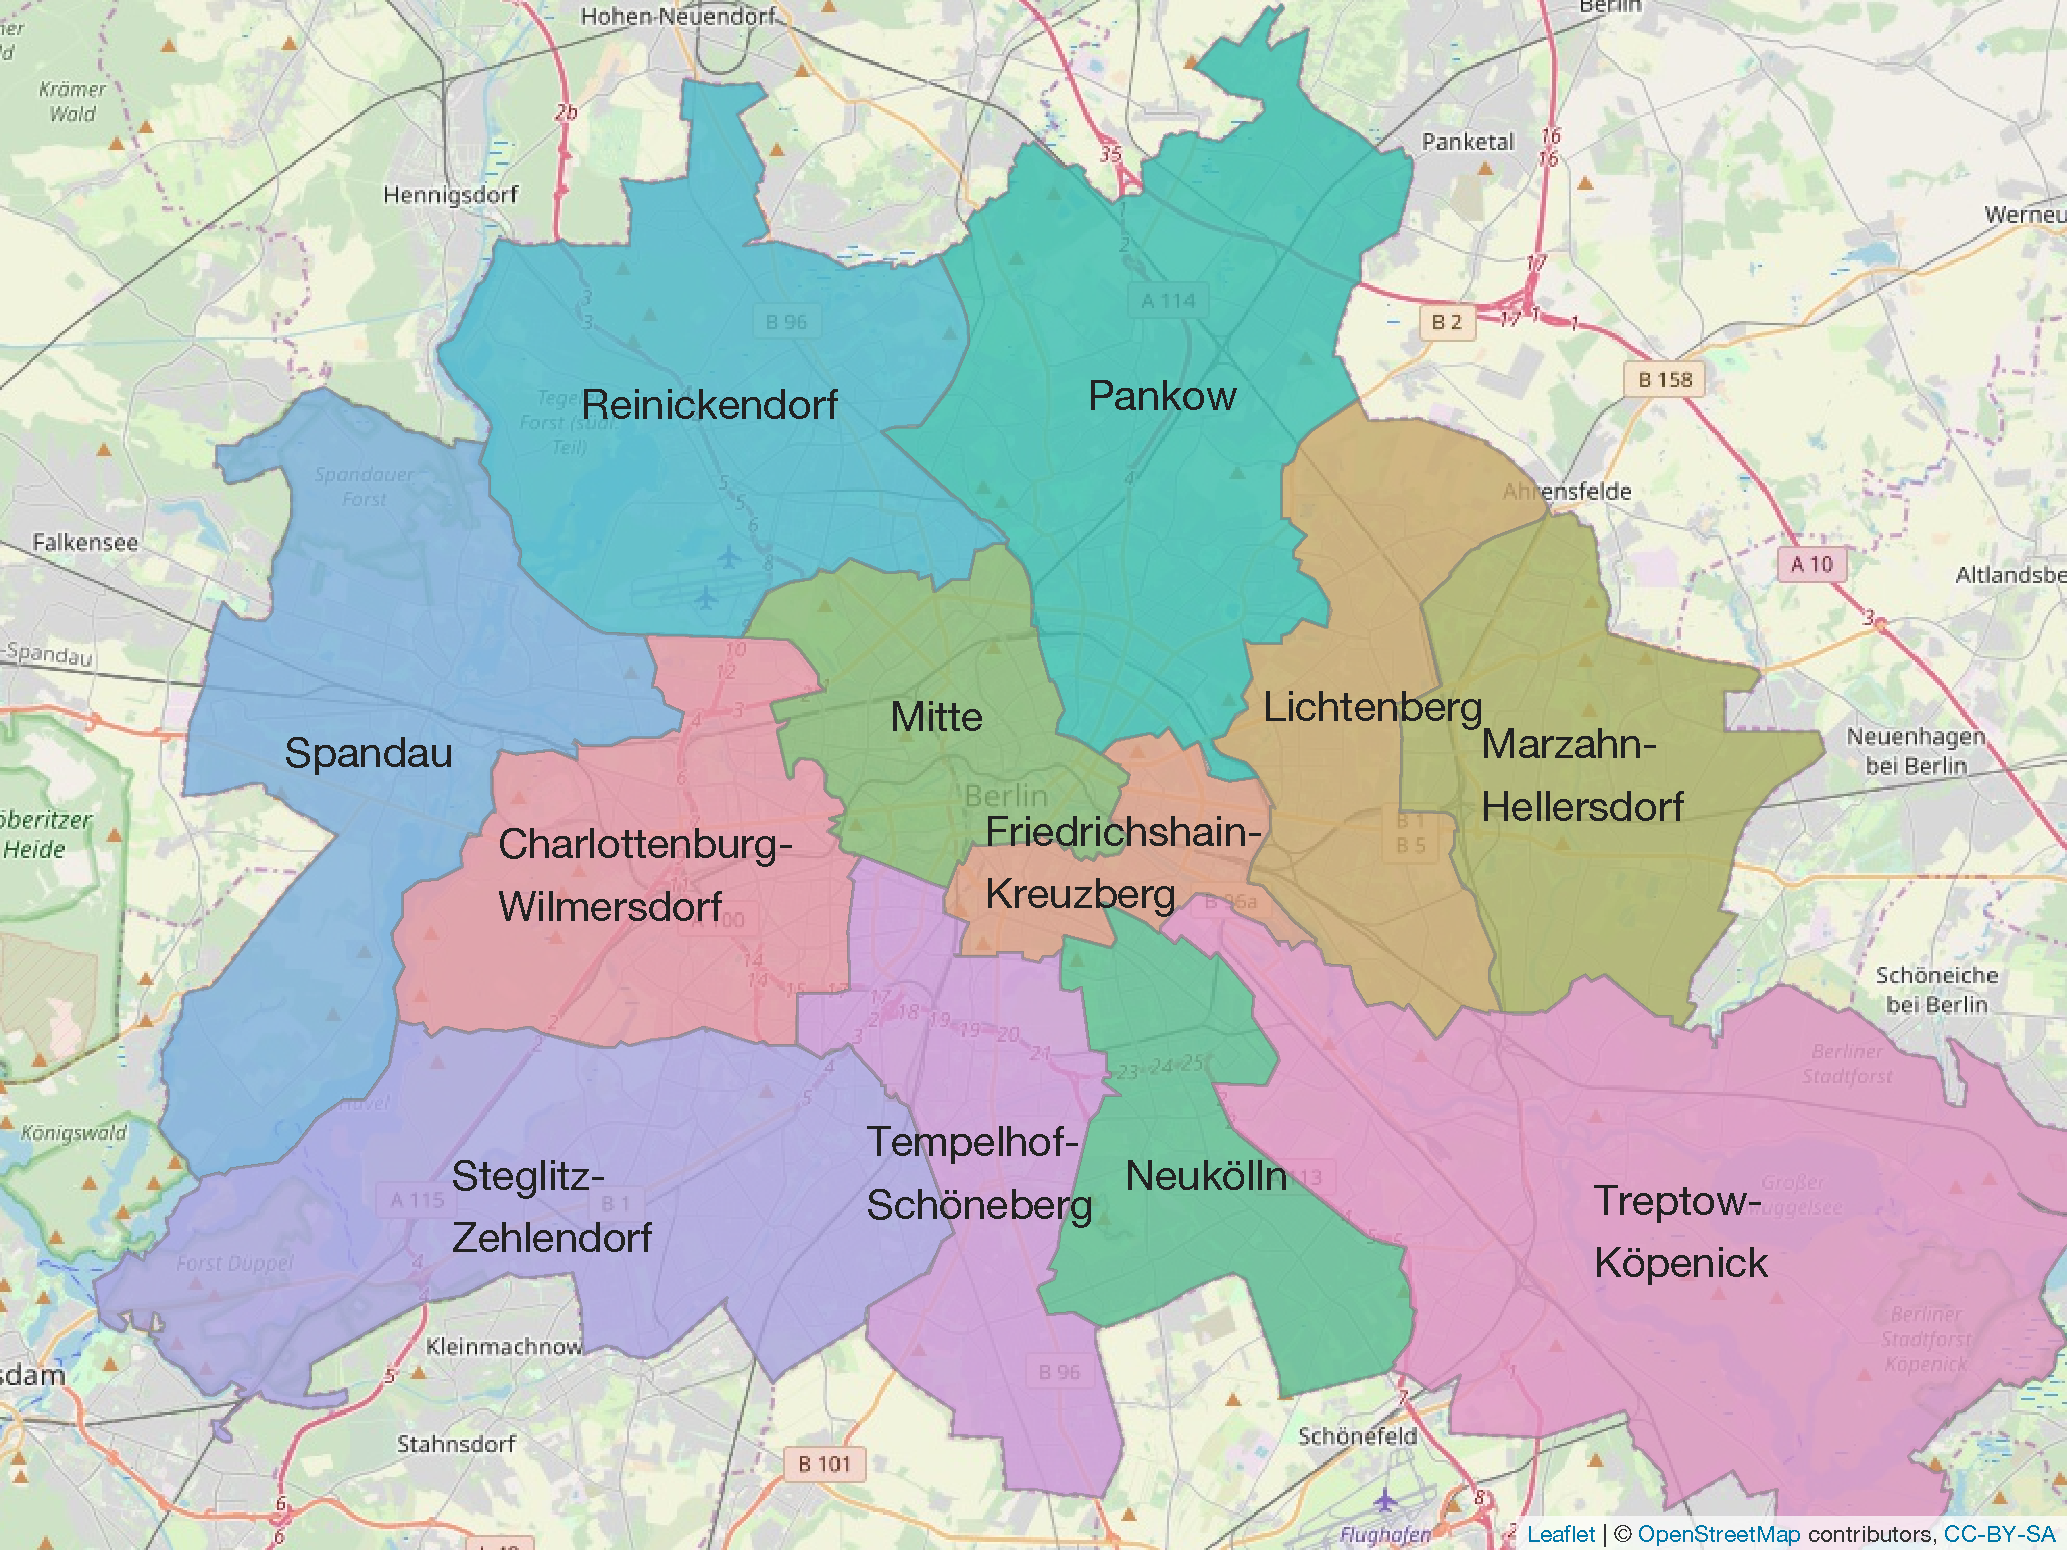
\includegraphics[height=1.8in]{berlin_district_leaflet.pdf}}
\subfloat[With \texttt{ggplot}]{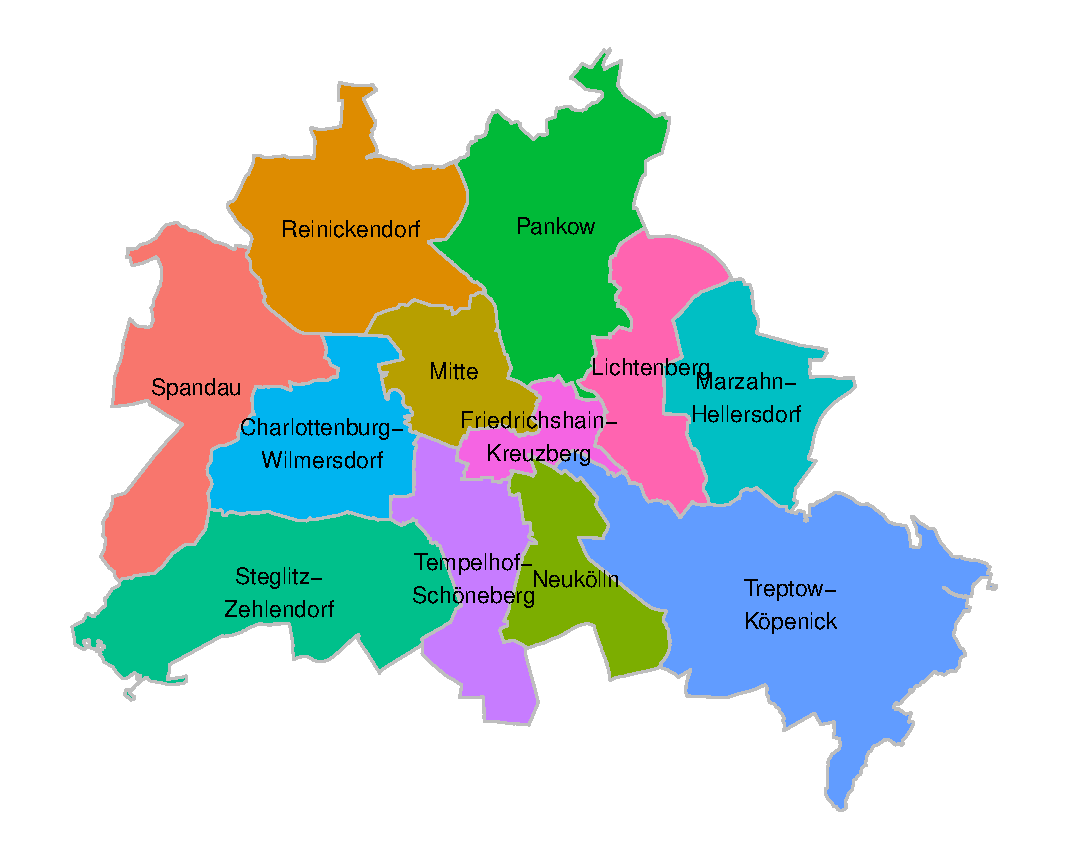
\includegraphics[height=1.8in]{berlin_district_ggplot.pdf}}
\caption{Maps of the Berlin Districts \protect
\includegraphics[scale=0.05]{qletlogo.pdf} {\href{https://github.com/silvia-ventoruzzo/SPL-WISE-2018/blob/master/Berlin_Districts_Neighbourhoods/berlin_districts_neighbourhoods_maps.R}{berlin\_districts\_neighbourhoods\_maps.R}}}
\centering
\end{figure}

\subsection{Berlin VBB Areas}

The VBB (Verkehrsverbund Berlin-Brandenburg) is "the public transport authority covering the federal states of Berlin and Brandenburg" (CITATION: \href{https://www.vbb.de/en/about-us/the-company-vbb}{VBB Website}). The city of Berlin, in particular, is divided in two fare areas: A, covering the center of Berlin up to the Ringbahn (circular line), and B, from the Ringbahn to the border with Brandenburg. After that there is also the area C, which however will not be covered here since we only consider the city of Berlin.

\begin{figure}[H]
\begin{center}
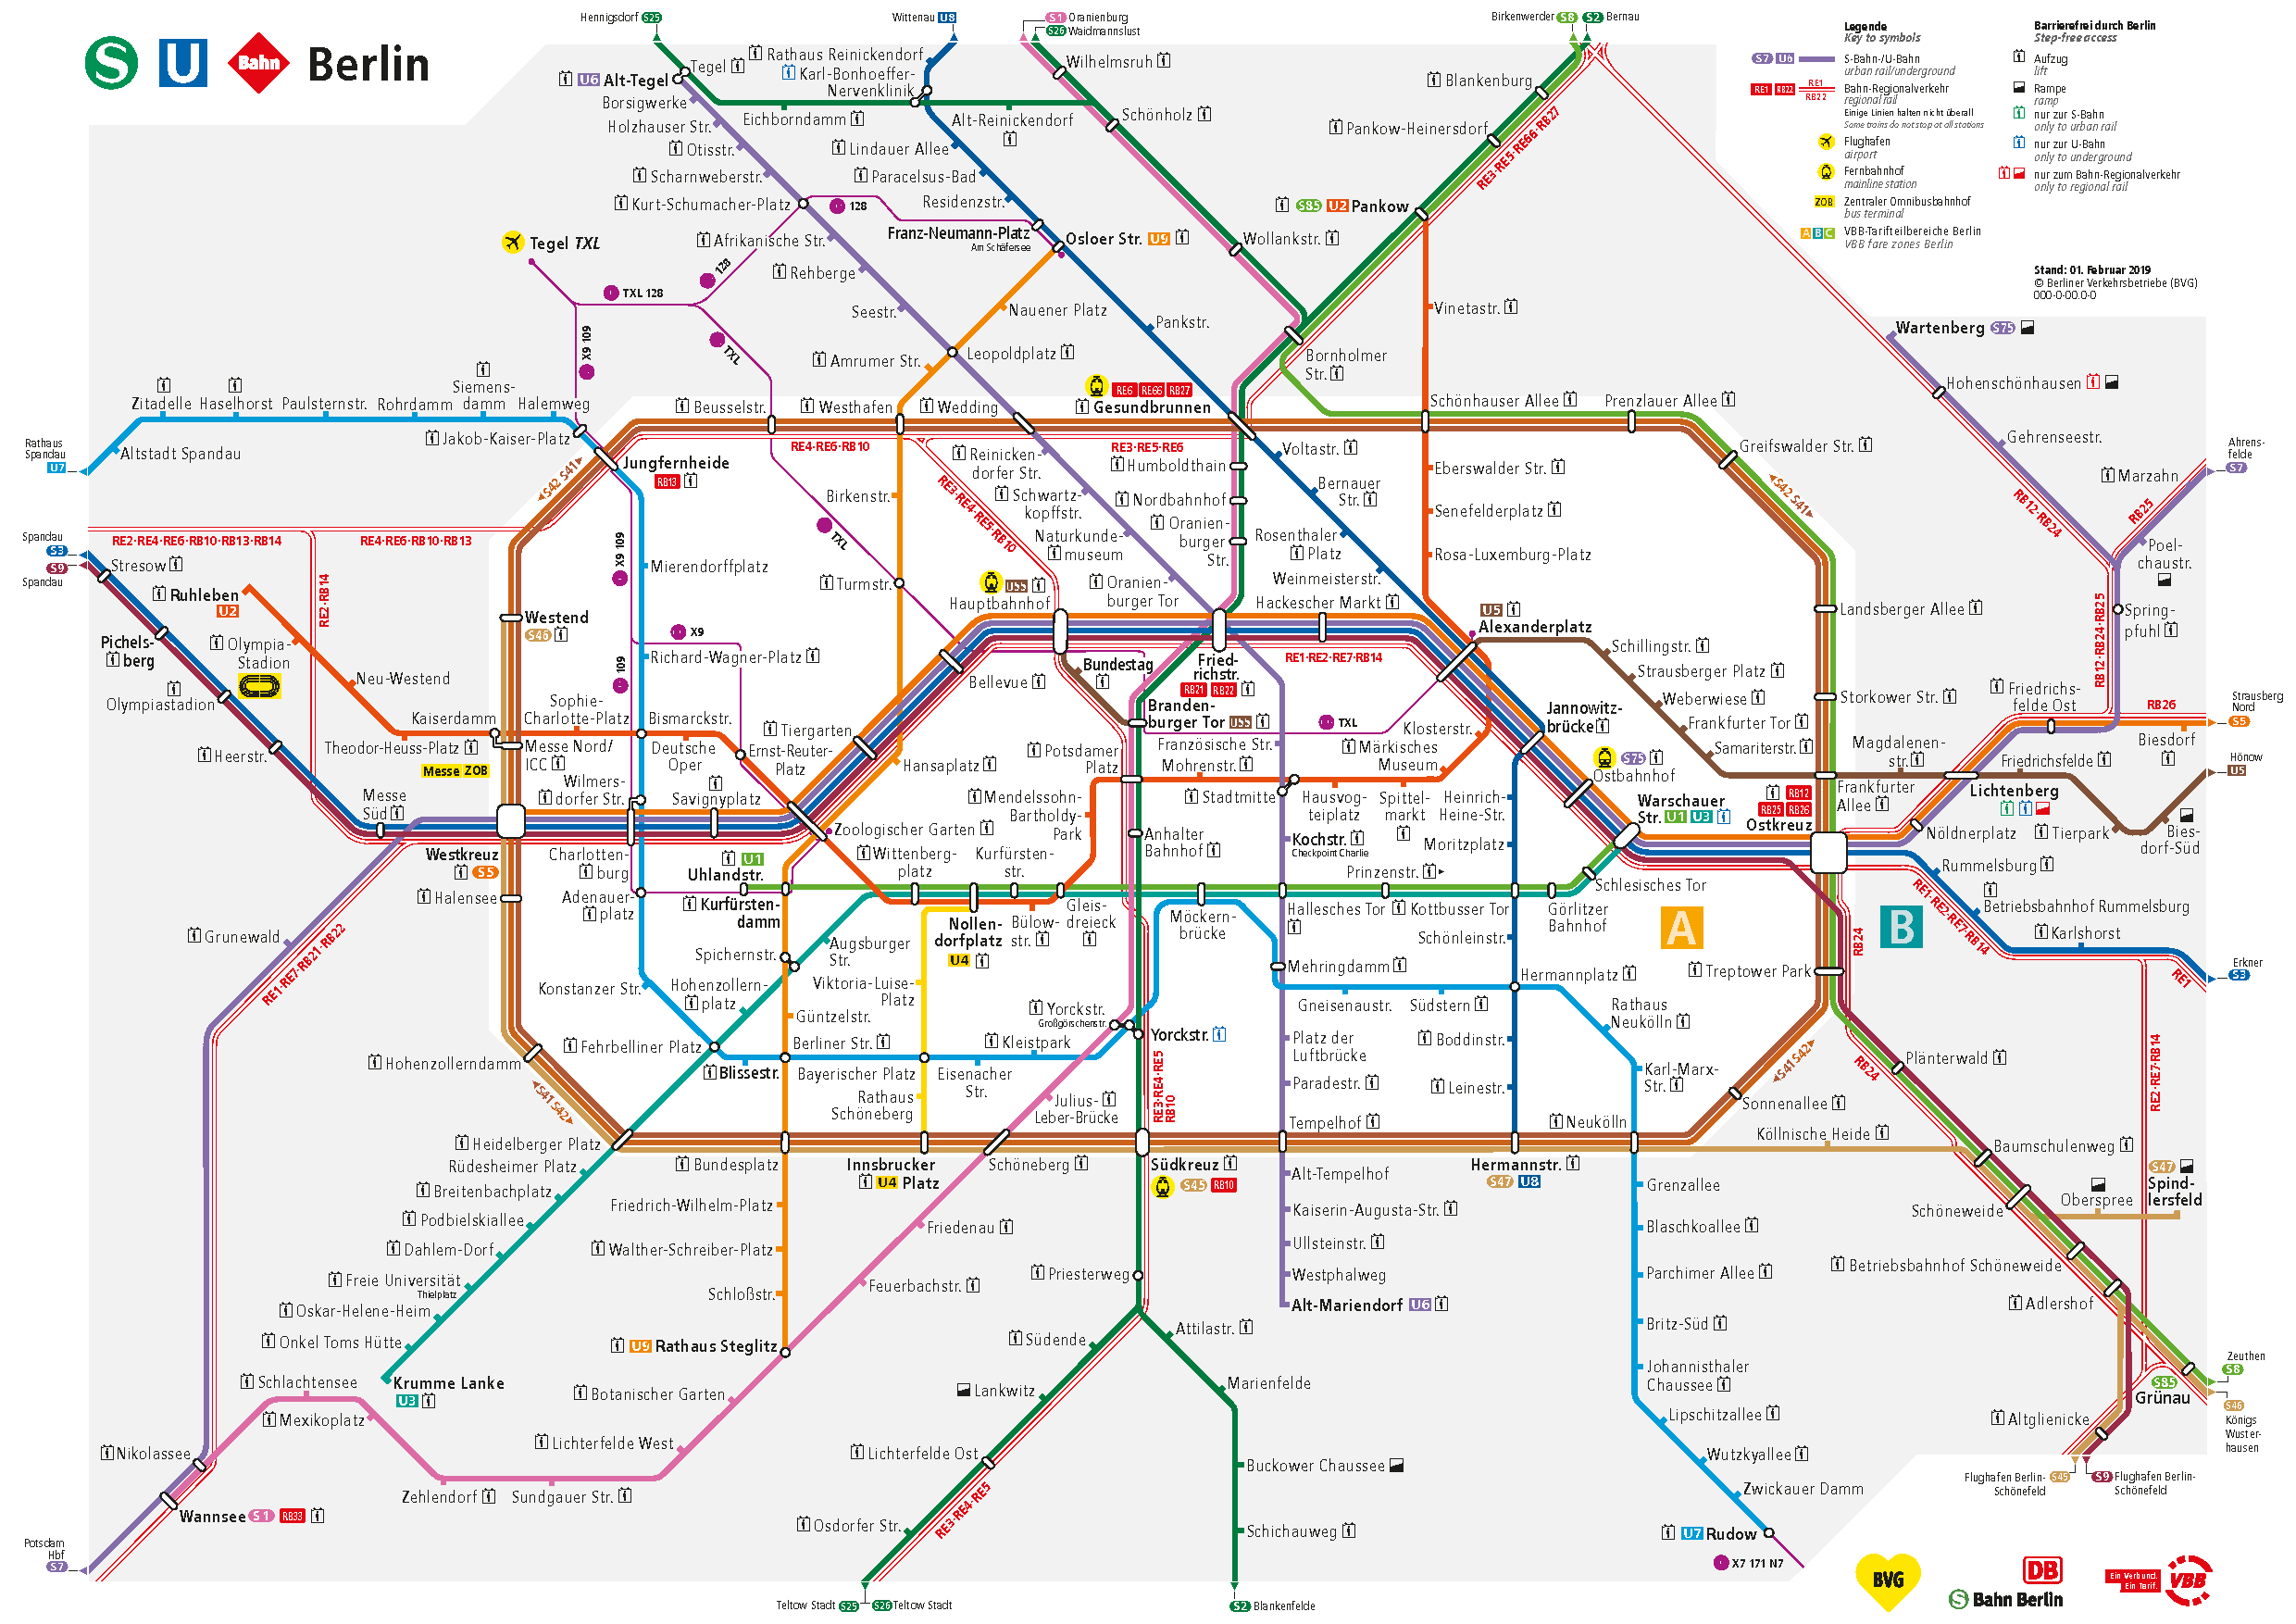
\includegraphics[width=0.8\textwidth, keepaspectratio]{S_und_U-Bahnnetz_mit_Regionalbahn_Innenstadt.pdf} \\
\caption{Network Map of Berlin Areas A and B (from \href{https://www.vbb.de/en/timetables/network-maps}{VBB Website})}
\end{center}
\end{figure}

We tried to replicate these areas by using the Berlin polygons and the stations points, which are again loaded using \texttt{st\_read} from the \texttt{sf} package.

\lstinputlisting[language=R, firstline=18, lastline=19, firstnumber=1, escapechar=|, caption={|\textbf{\href{https://github.com/silvia-ventoruzzo/SPL-WISE-2018/blob/master/Berlin_VBB_Areas/berlin_vbb_areas.R}{berlin\_vbb\_areas.R}}|}]{../Berlin_VBB_Zones/berlin_vbb_zones.R}

First of all, we need to create the polygon for area A. This is done by joining the points and transforming this into a polygon.

Firstly, we filter the stations that belong to the Ringbahn (border of area A). Since the shapefile does not include the line name for the stations, we need to create our own vector of names. We also add the order in which they need to be connected. The first and last station are the same since the circle need to close.

\lstinputlisting[language=R, firstline=22, lastline=33, firstnumber=1, escapechar=|, caption={|\textbf{\href{https://github.com/silvia-ventoruzzo/SPL-WISE-2018/blob/master/berlin_vbb_zones/berlin_vbb_zones.R}{berlin\_vbb\_areas.R}}|}]{../Berlin_VBB_Zones/berlin_vbb_zones.R}

Since some stations appear multiple time, being both subway and lightrail stations (and maybe even bus and tram stops), we filter railway stations, which include both subway and lightrail, and then we calculate the middle point for each station among the ones having the same name.

\lstinputlisting[language=R, firstline=36, lastline=44, firstnumber=1, escapechar=|, caption={|\textbf{\href{https://github.com/silvia-ventoruzzo/SPL-WISE-2018/blob/master/Berlin_VBB_Zones/berlin_vbb_zones.R}{berlin\_vbb\_areas.R}}|}]{../Berlin_VBB_Zones/berlin_vbb_zones.R}

By performing a right join with the dataframe with the Ringbahn station names, we only keep these stations. After performing some preparation steps, we use the function \texttt{st\_polygon} from the \texttt{sf} package, which creates a polygon out of a list of points (CHECK!!!).

\lstinputlisting[language=R, firstline=45, lastline=52, firstnumber=11, escapechar=|, caption={|\textbf{\href{https://github.com/silvia-ventoruzzo/SPL-WISE-2018/blob/master/Berlin_VBB_Zones/berlin_vbb_zones.R}{berlin\_vbb\_areas.R}}|}]{../Berlin_VBB_Zones/berlin_vbb_zones.R}

Secondly we need to create a polygon for entire Berlin. This is done by simply uniting all the neighbourhoods.

\lstinputlisting[language=R, firstline=55, lastline=56, firstnumber=19, escapechar=|, caption={|\textbf{\href{https://github.com/silvia-ventoruzzo/SPL-WISE-2018/blob/master/Berlin_VBB_Zones/berlin_vbb_zones.R}{berlin\_vbb\_areas.R}}|}]{../Berlin_VBB_Zones/berlin_vbb_zones.R}

Finally, we bind the two objects by rows and calculate their intersections thanks to the function \texttt{st\_intersection}. We then define the area names according to how many times the two previous polygons intersect:
	\begin{itemize}
    		\item Area A: where polygons intersect (n. overlaps > 1)
    		\item Area B: where polygons do not intersect (n. overlaps $\leq$ 1)
    \end{itemize}

\lstinputlisting[language=R, firstline=59, lastline=64, firstnumber=21, escapechar=|, caption={|\textbf{\href{https://github.com/silvia-ventoruzzo/SPL-WISE-2018/blob/master/Berlin_VBB_Zones/berlin_vbb_zones.R}{berlin\_vbb\_areas.R}}|}]{../Berlin_VBB_Zones/berlin_vbb_zones.R}

In this code the custom-function \texttt{points\_midpoint} was used to calculate the middle point among many. It extracts the coordinates of the points thanks to \texttt{st\_coordinates} and then calculates the mean of latitude and longitude.

\lstinputlisting[language=R, firstline=2, escapechar=|, caption={|\textbf{\href{https://github.com/silvia-ventoruzzo/SPL-WISE-2018/blob/master//Helpers/points_midpoint.R}{points\_midpoint.R}}|}]{../Berlin_VBB_Zones/Helpers/points_midpoint.R}

This sf object can be used to map the VBB zones using \texttt{leaflet} or \texttt{ggplot2}.

\begin{figure}[H]
\centering
\subfloat[With \texttt{leaflet}]{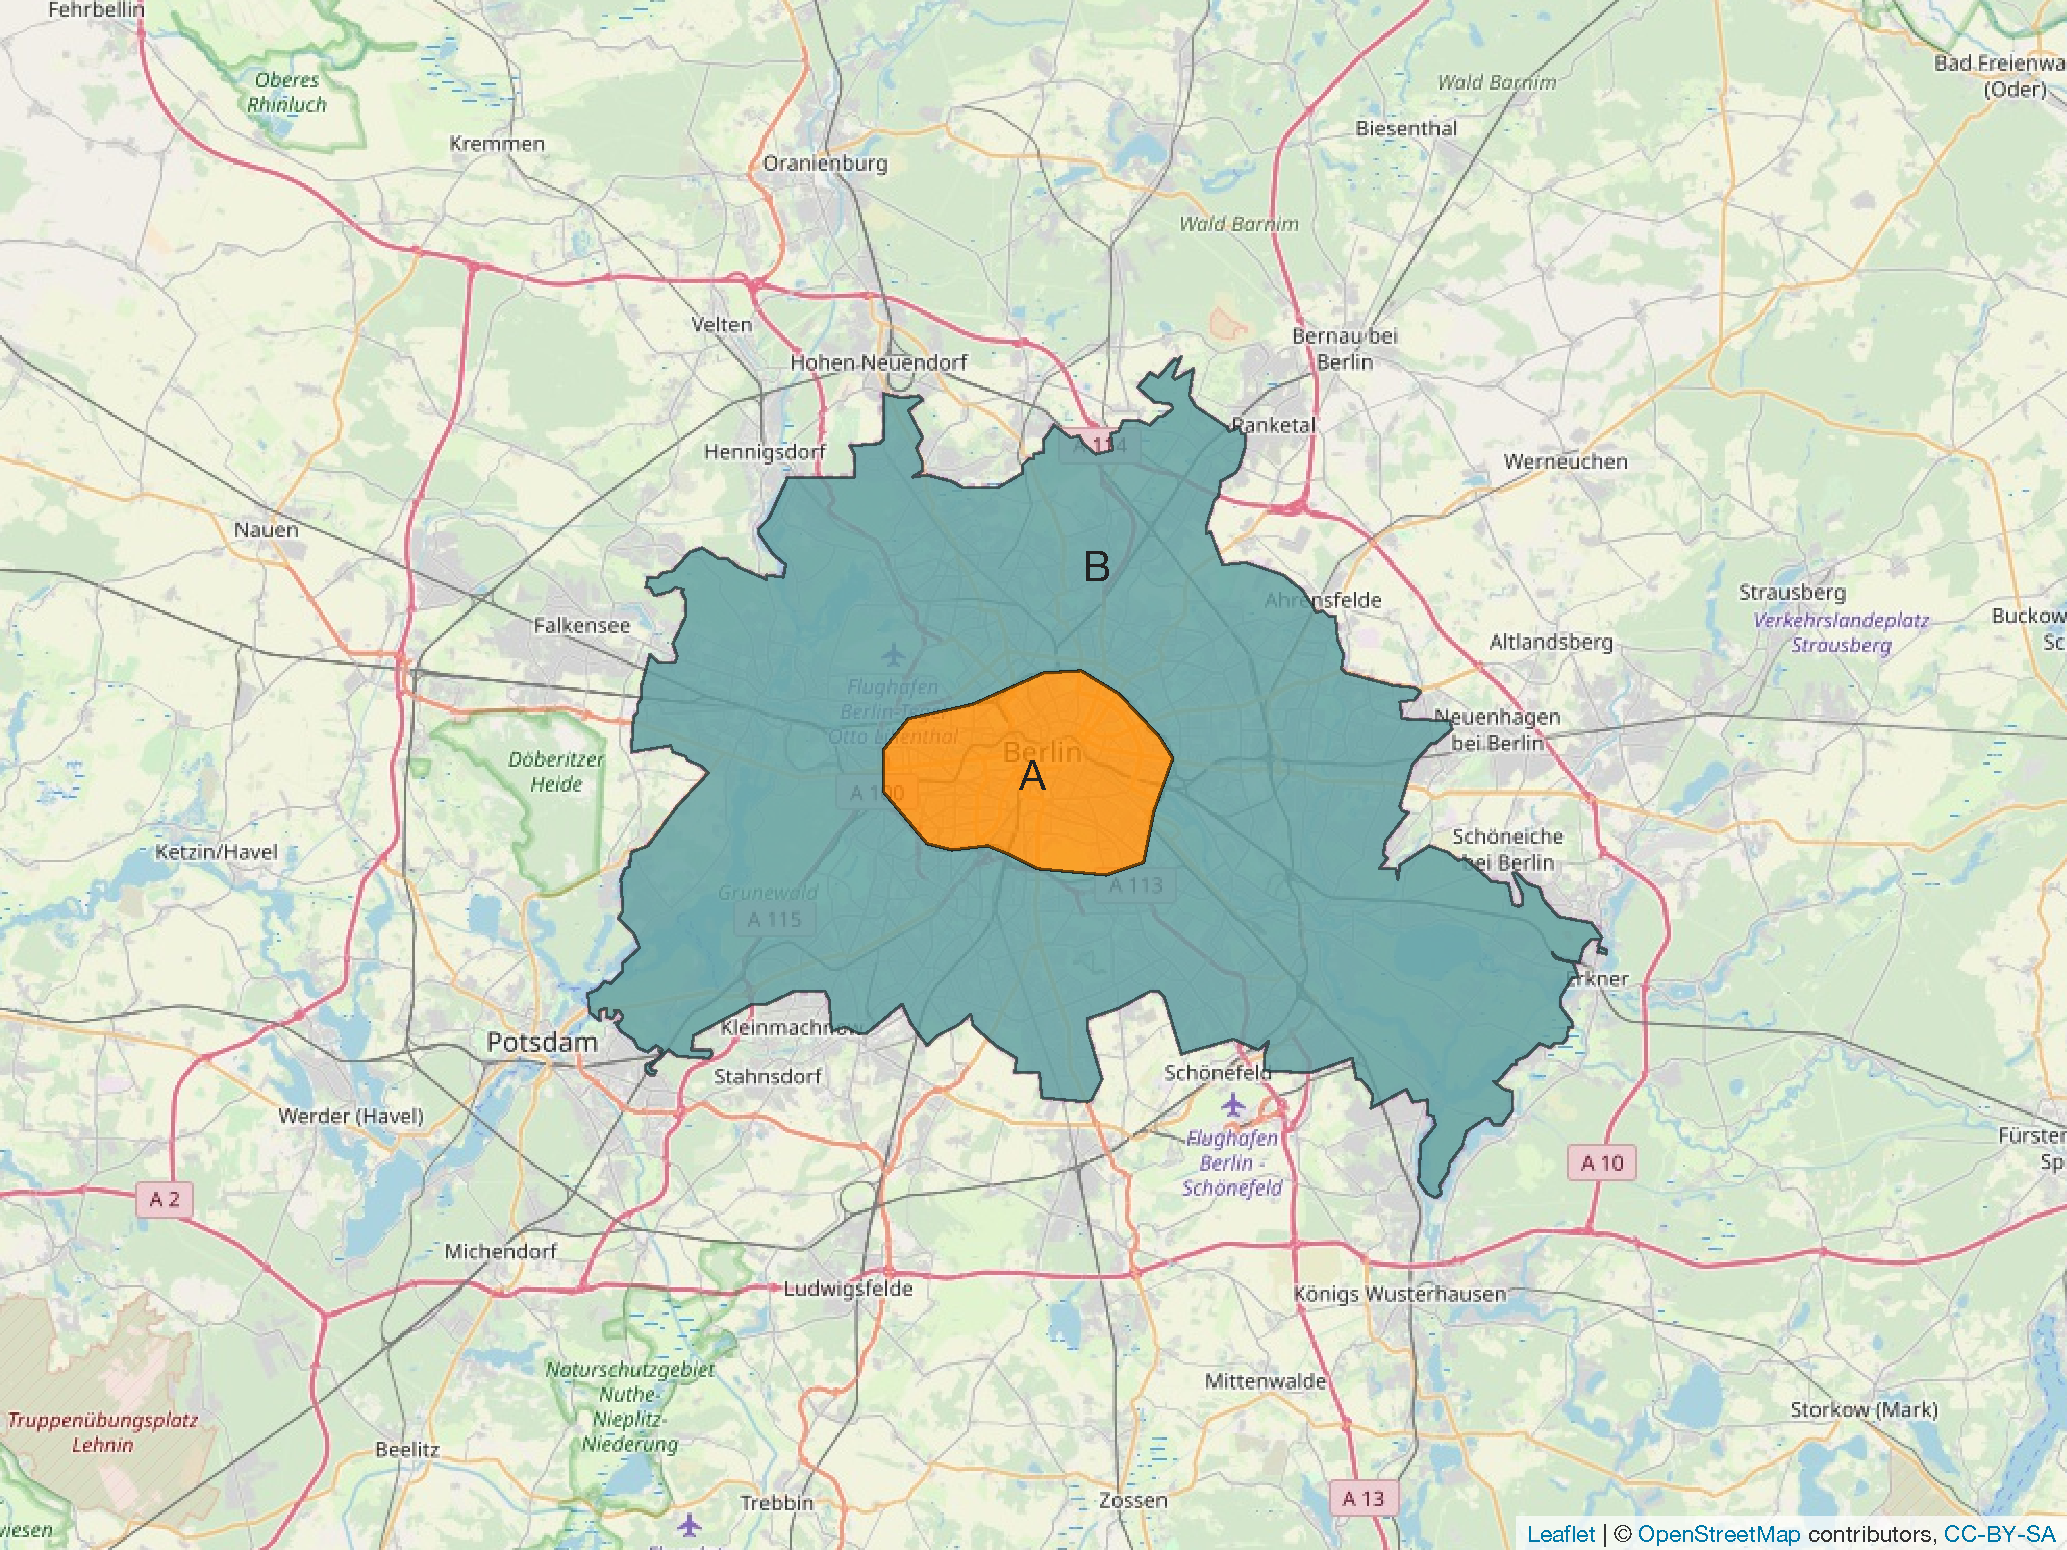
\includegraphics[height=1.8in]{berlin_vbb_zones_leaflet.pdf}}
\subfloat[With \texttt{ggplot}]{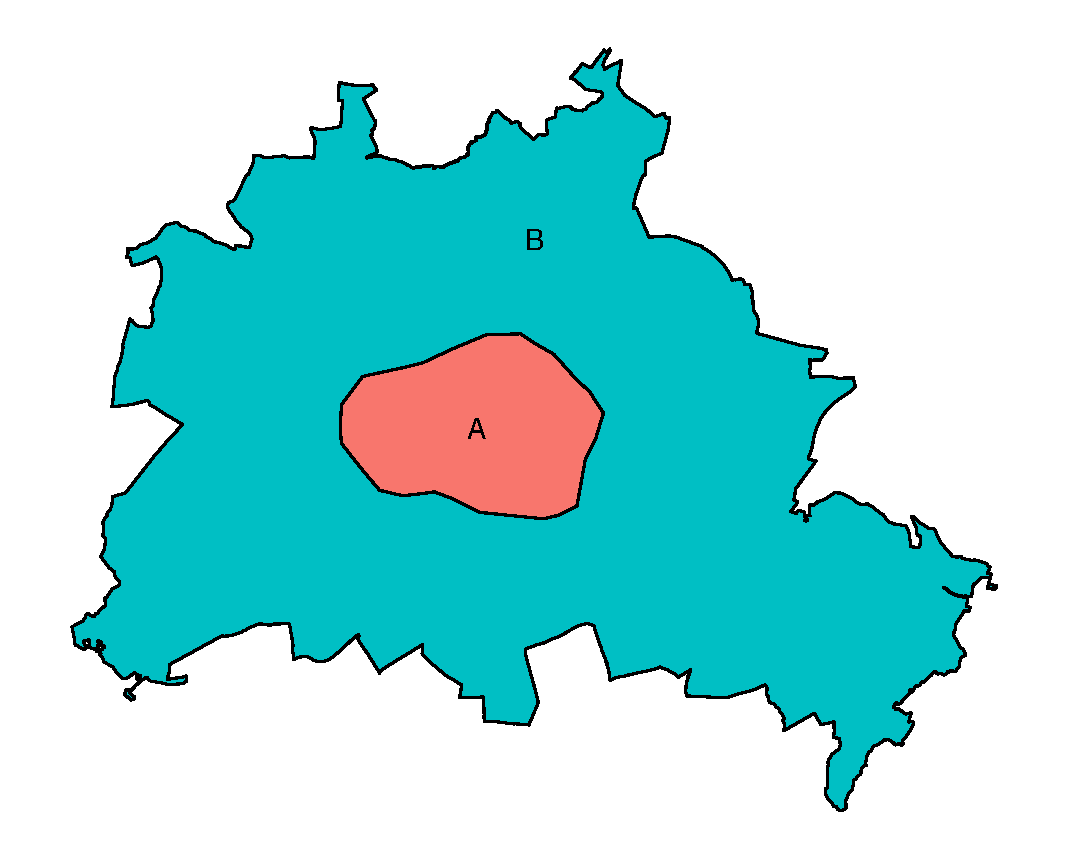
\includegraphics[height=1.8in]{berlin_vbb_zones_ggplot.pdf}}
\caption{Maps of the Berlin VBB Zones \protect
\includegraphics[scale=0.05]{qletlogo.pdf} {\href{https://github.com/silvia-ventoruzzo/SPL-WISE-2018/blob/master/Berlin_VBB_Zones/berlin_vbb_zones_maps.R}{berlin\_vbb\_zones\_maps.R}}}
\centering
\end{figure}

\subsection{Airbnb listings' attributes}

The first part of cleaning the airbnb datasets consists in joining the two containing general information according to their common variables and correcting some string values.
Secondly, we proceed in checking for missing values and deriving that information from other correlated variables.
Thirdly, we proceed to feature engineering.
We firstly derive the areas where they are located thanks to the spatial polygons created before and the function \texttt{point\_in\_polygons}.

\lstinputlisting[language=R, firstline=2, escapechar=|, caption={|\textbf{\href{https://github.com/silvia-ventoruzzo/SPL-WISE-2018/blob/master/Helpers/point_in_polygons.R}{point\_in\_polygons.R}}|}]{../Helpers/point_in_polygons.R}

This function loops through the polygons in the \texttt{sf} object and check which points are contained in which polygons. In the end it writes the id associated to the polygon, in our case the area id, in the summary column, which can be named as preferred.

Secondly, for railway stations and tourist attractions we calculate the amount inside a range and the distance to the nearest point using the function \texttt{distance\_count}. In particular, the following parameters will be used:

\begin{itemize}

    \item Railway stations: distance = 1000 (1 km)

    \item (Top 10) attractions: distance = 2000 (2 km)
    
\end{itemize}

\lstinputlisting[language=R, firstline=3, escapechar=|, caption={|\textbf{\href{https://github.com/silvia-ventoruzzo/SPL-WISE-2018/blob/master/Helpers/distance_count.R}{distance\_count.R}}|}]{../Helpers/distance_count.R}

This function firstly calculates the distance between all properties and all reference points, railway stations or tourist attractions, using the Haversine Formula, which "gives  minimum  distance  between  any  two  points  on  spherical body by using latitude and longitude" \citep{haversine:2013}.

\begin{equation}
d = 2r \arcsin \Bigg(\sqrt{\sin^2\Big(\frac{\phi_2 - \phi_1}{2}\Big) + \cos(\phi_2)\cos(\phi_1)\sin^2\Big(\frac{\psi_2 - \psi_1}{2}\Big)}\Bigg)
\end{equation}

%% \mathrm{where} \phi \mathrm{corresponds to the latitude and} \psi \mathrm{to the longitude of the two points.}



\iffalse

\begin{table}[H]
\centering
\begin{tabular}{l}
  \hline
x \\ 
  \hline
id \\ 
  attraction\_count \\ 
  attraction\_dist \\ 
  station\_count \\ 
  station\_dist \\ 
  long \\ 
  lat \\ 
  price \\ 
  property\_type \\ 
  room\_type \\ 
  security\_deposit\_yn \\ 
  cleaning\_fee\_yn \\ 
  host\_is\_superhost \\ 
  accommodates \\ 
  bedrooms \\ 
  beds \\ 
  minimum\_nights \\ 
  review\_scores\_rating \\ 
  number\_of\_reviews \\ 
  reviewed\_yn \\ 
  cancellation\_policy \\ 
  availability\_30 \\ 
  availability\_60 \\ 
  availability\_90 \\ 
  availability\_365 \\ 
  listing\_url \\ 
  district \\ 
  vbb\_area \\ 
  neighbourhood \\ 
  2018\_fall\_availability \\ 
  2018\_winter\_availability \\ 
  2019\_spring\_availability \\ 
  2019\_summer\_availability \\ 
  2019\_fall\_availability \\ 
  2019\_winter\_availability \\ 
   \hline
\end{tabular}
\end{table}

\fi




\section{Exploratory Data Analysis}\label{Sec:Exploratory}

The exploratory data analysis will be divided in two parts: subsection \ref{subsec:descriptive} will show the descriptive statistics calculated either numeric or categorical variables; subsection \ref{subsec:distrplots} will then display the distribution plots. 
Correlation will also be calculated, but only with respect to price. This subject will be dealt with in subsection \ref{subsec:corr}.

\subsection{Descriptive statistics}\label{subsec:descriptive}

Descriptive statistics make the interpretation of the data easier by giving grouping it and thus providing a shorter representation of it \citep{descrstat:2014}.

As in \cite{descrstat:2014} explained there are three general types of descriptive statistics:
\begin{enumerate}
\item Measures of central tendency
\item Measures of spread
\item Graphical displays
\end{enumerate}

This subsection will focus on the first two, while subsection 
\ref{subsec:distrplots} will deal with the third.

Most of these statistics are usually applied to continuous data, sometimes even to numerical discrete data, but not to categorical variables. Therefore the function to calculate descriptive statistics has been split in two.

The first part calculate both measures of central tendency and spread of all numerical variables thanks to the function \texttt{apply}. The function \texttt{apply(X, MARGIN, FUN, ...)} calculates the function in \texttt{FUN} for all rows (\texttt{MARGIN = 1}) or columns (\texttt{MARGIN = 2}) for the data in \texttt{X}. One can add additional arguments, like the quantile probabilites in our case.


\lstinputlisting[language=R, firstline=1, lastline=17, firstnumber=1, escapechar=|, caption={|\textbf{\href{https://github.com/silvia-ventoruzzo/SPL-WISE-2018/blob/master/Helpers/descriptive_statistics.R}{descriptive\_statistics.R}}|}]{../Helpers/descriptive_statistics.R}

Part of the results can be seen in table \ref{table:descrstatnum}.



\begin{table}[H]
\centering
\begin{tabular}{lrrrrrrrr}
  \hline \hline
variable & min & 1Q & median & 3Q & max & iqr & mean & sd \\ 
  \hline
price & 0.00 & 30.00 & 45.00 & 70.00 & 9000.00 & 40.00 & 67.14 & 220.28 \\ 
   \hline \hline
\end{tabular}
\caption{Sample of descriptive table for numeric variables}
\label{table:descrstatnum}
\end{table}

For categorical variables the explained statistics do not work, therefore frequencies and proportions of each factor were calculated.

\lstinputlisting[language=R, firstline=20, lastline=50, firstnumber=19, caption={|\textbf{\href{https://github.com/silvia-ventoruzzo/SPL-WISE-2018/blob/master/Helpers/descriptive_statistics.R}{descriptive\_statistics.R}}|}]{../Helpers/descriptive_statistics.R}


\subsection{Distribution plots}\label{subsec:distrplots}

Also for the distribution plots we distinguish between numerical and categorical variables. In the first case a density plot has been produced, where also mean, median, 1st and 3rd quantiles are visible.
Unfortunately, many variables present outliers, which were in some cases excluded from the plots for better visualization.

\begin{figure}[H]
\centering
\subfloat[Complete]{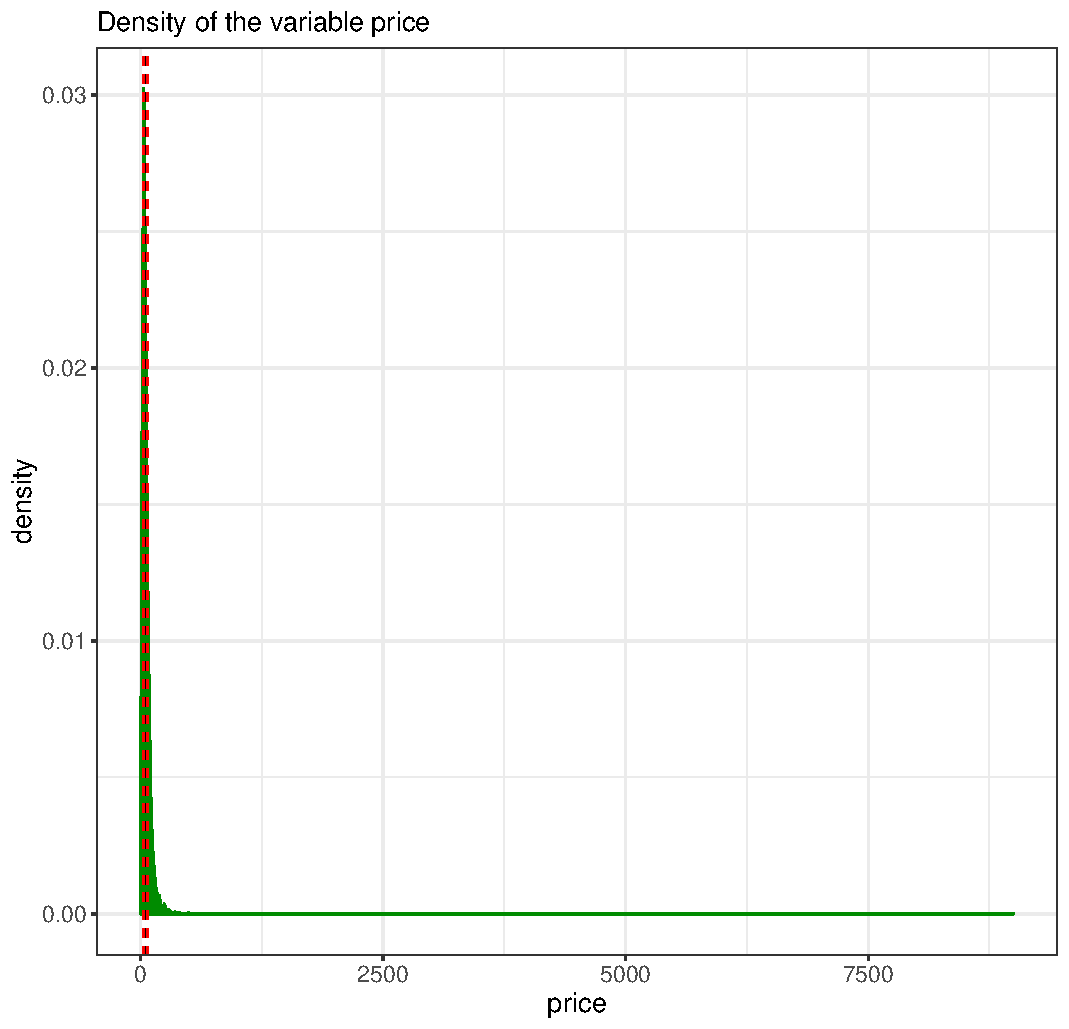
\includegraphics[height=7cm]{price_distribution_complete.pdf}}
\subfloat[Without outliers]{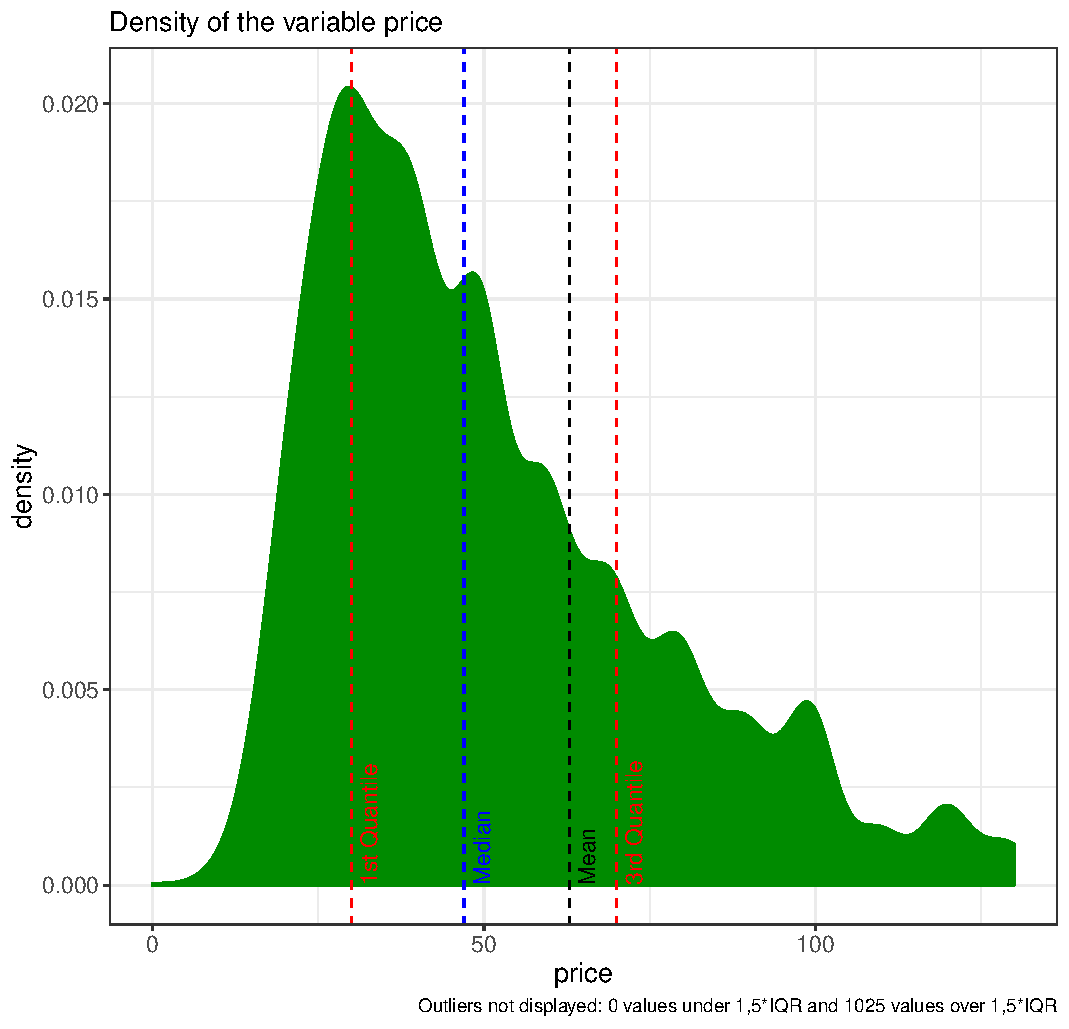
\includegraphics[height=7cm]{price_distribution_nooutliers.pdf}}
\caption{Distribution of the variable price \protect
\includegraphics[scale=0.05]{qletlogo.pdf} {\href{https://github.com/silvia-ventoruzzo/SPL-WISE-2018/blob/master/exploratory_data_analysis.R}{exploratory\_data\_analysis.R}}}
\centering
\end{figure}

For the categorical variables a bar plot is more appropriate, since the values that the variable can assume are discrete and usually also few, like in the case displayed in figure \ref{figure:room_type}.




\begin{figure}[H]
\begin{center}
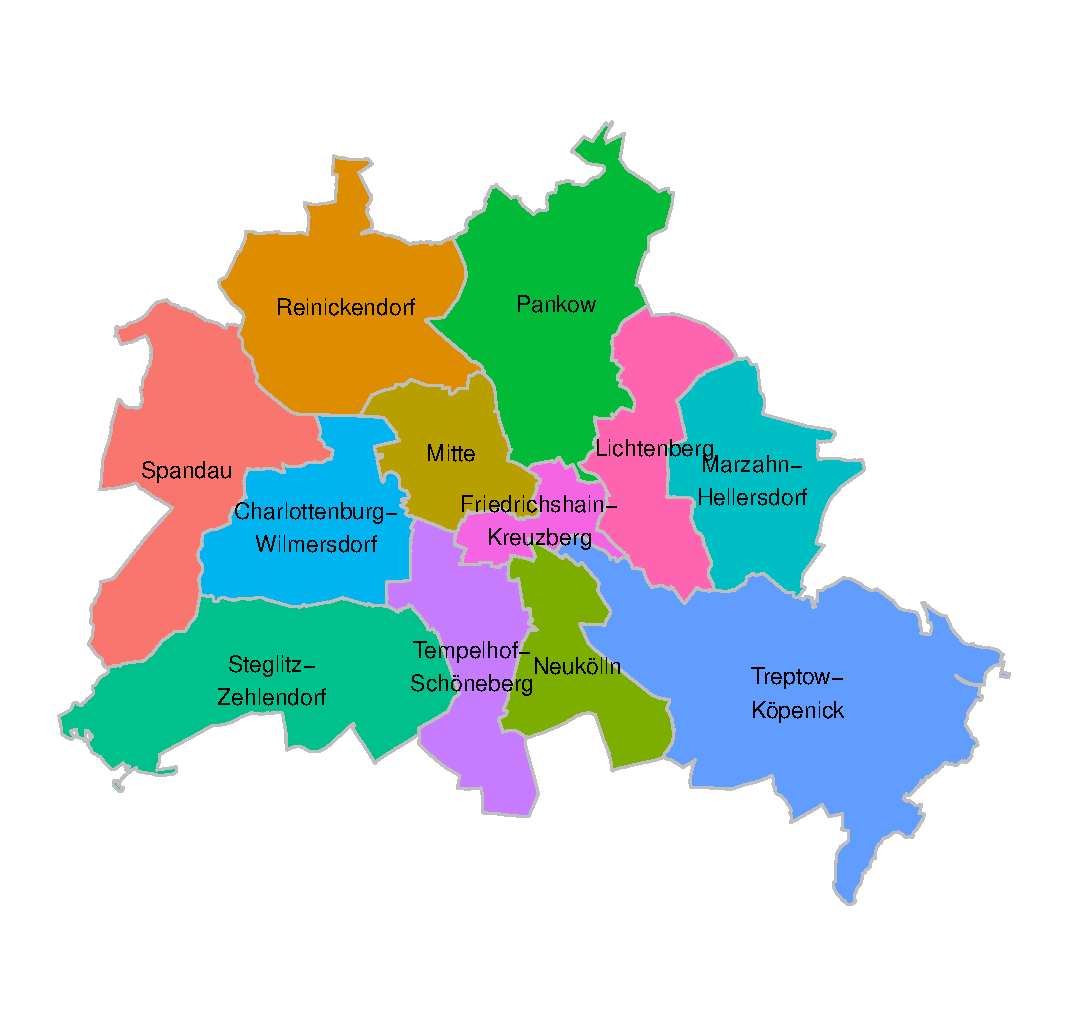
\includegraphics[width=0.5\textwidth, keepaspectratio]{room_type_distribution.pdf} \\
\caption{Distribution of the variable room\_type \protect
\includegraphics[scale=0.05]{qletlogo.pdf} {\href{https://github.com/silvia-ventoruzzo/SPL-WISE-2018/blob/master/exploratory_data_analysis.R}{exploratory\_data\_analysis.R}}}
\label{figure:room_type}
\end{center}
\end{figure}

We also mapped the Berlin districts and the distribution of the average of a certain variable on them with the use of the package \textit{leaflet}.

\begin{figure}[H]
\begin{center}
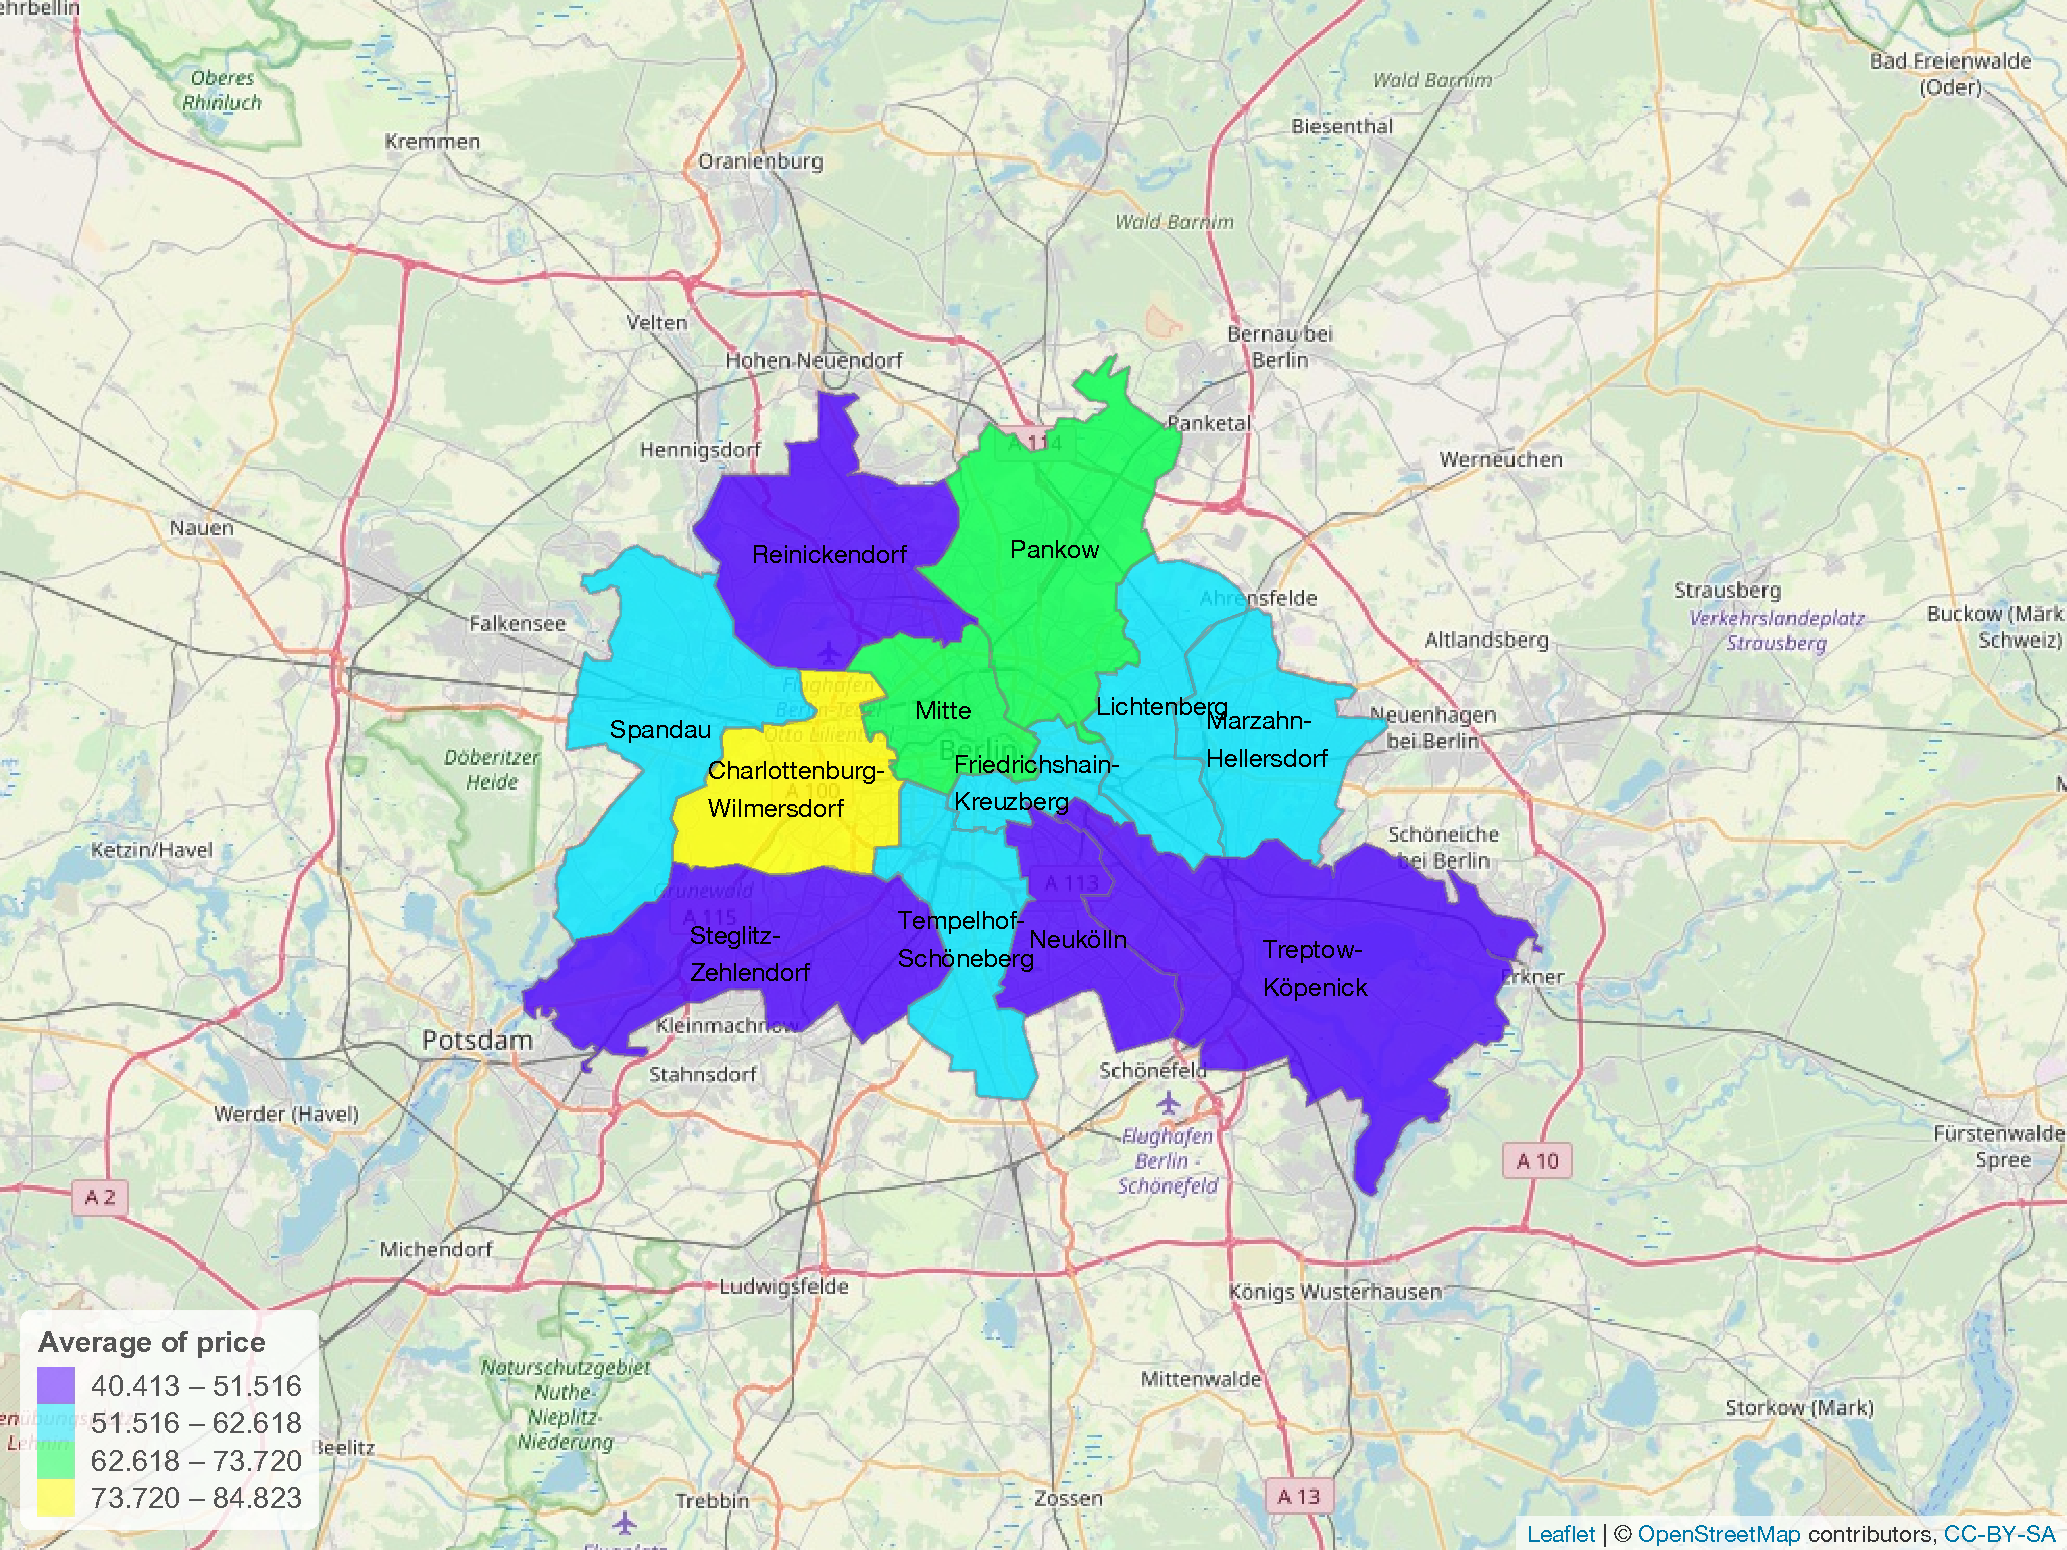
\includegraphics[width=0.5\textwidth, keepaspectratio]{price_map_distr} \\
\caption{Distribution of the average of price across Berlin's districts}
\label{figure:room_type}
\end{center}
\end{figure}
\newpage
\section{Price analysis}\label{Sec:Price analysis}

One of the core factors in the choice of the property to book is its price, being one of main drivers of customers' behaviors \citep{liang2018understanding}. Therefore one may want to try and see what properties' attributes influence its value.

We start in subsection \ref{subsec:corr} by calculating the correlation of all the other variables with respect to price. Then we try in subsection \ref{subsec:lm} to run a linear regression on price to look what variables are statistically relevant and how much they affect the price.


\subsection{Correlation with price}\label{subsec:corr}

Since we are only interested in the correlation with price, a classic correlation plot like the one produced by \texttt{corrplot} from the package \texttt{corrplot} may not be the most easily readable in this case, especially because of the large number of variables.

In fact, categorical variables first need to be transformed into many dummy variables in order to calculate the correlation. The function \texttt{from\_row\_to\_col} will be used to achieve this result. It creates dummy variables for all factor levels by creating a column of 1s, spreading it across so many columns as factor levels and filling the empty rows in the columns with 0s.

\lstinputlisting[language=R, firstline=2, escapechar=|, caption={|\textbf{\href{https://github.com/silvia-ventoruzzo/SPL-WISE-2018/blob/master/Helpers/from_row_to_col.R}{from\_row\_to\_col.R}}|}]{../Helpers/from_row_to_col.R}


\begin{figure}[H]
\begin{center}
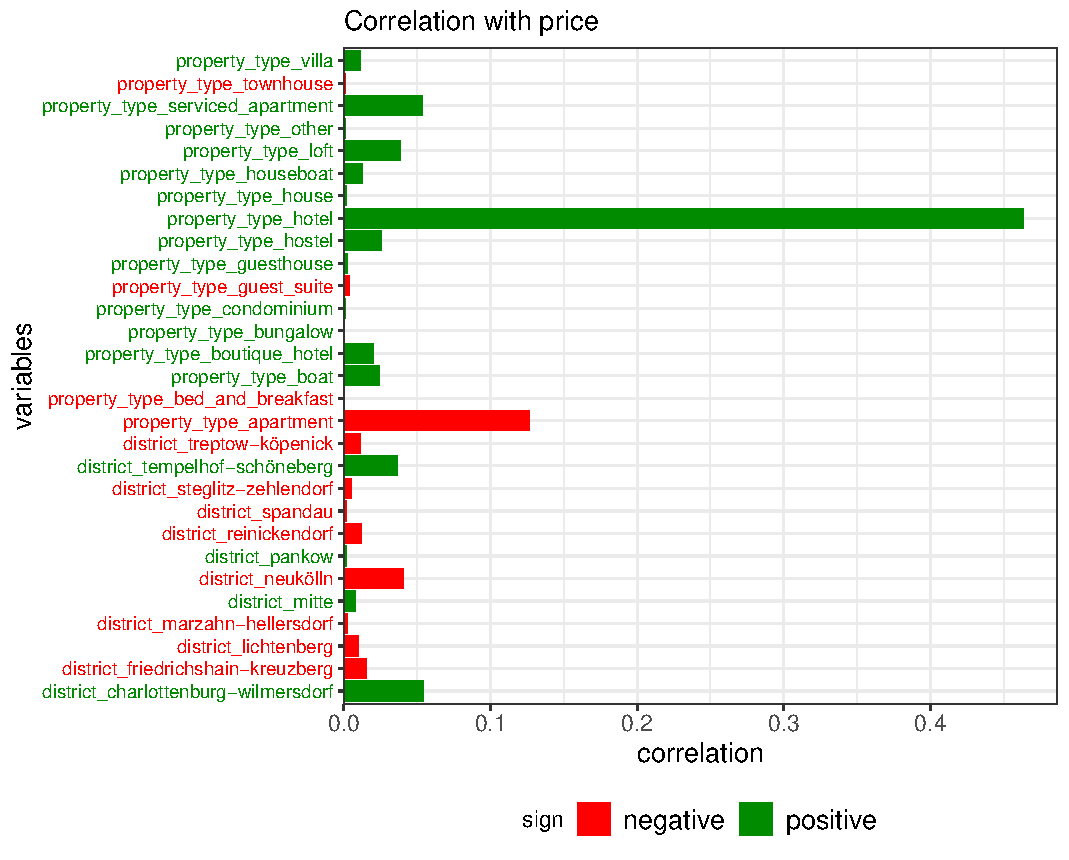
\includegraphics[width=0.8\textwidth, keepaspectratio]{price_correlation.pdf} \\
\caption{Sample of plot of correlation with price \protect
\includegraphics[scale=0.05]{qletlogo.pdf} {\href{https://github.com/silvia-ventoruzzo/SPL-WISE-2018/blob/master/Helpers/correlation_plot.R}{correlation\_plot.R}}}
\label{figure:pricecorr}
\end{center}
\end{figure}



\subsection{Linear regression on price}\label{subsec:lm}

As pointed out in \cite{wang2017price} linear regression is used to describe possible linear relationships between a dependent variable and one or multiple independent variables.

In this case we will look for the relationship that the properties' attributes have on their price. For this purpose we used again the data with the categorical variables transformed to dummies. The linear regression was then run using all other variables, except \textit{id}, \textit{long}, \textit{lat}, \textit{neighbourhood} and \textit{listing\_url}, as regressors.

On table \ref{table:lmresults} you can see a sample of the results. A positive coefficient means that the variable has a positive impact on the dependent variable, the higher this regressor is, the higher \textit{price} will be. On the other side, a negative coefficient suggests that a higher value of the independent variable will result in a lower value of \textit{price}. Moreover, a variable is considered significant if the p-value is lower than the significance level, set at 5\% in this case, since it rejects the null hypothesis for that regressor coefficient to be equal to zero \cite{moye2006statistical}.

\begin{table}[H]
\centering
\begin{tabular}{lrl}
  \hline
variable & coefficient & significant \\ 
  \hline
(Intercept) & 12.69 & FALSE \\ 
  host\_listings\_count & -0.73 & TRUE \\ 
  accommodates & 16.31 & TRUE \\ 
   \hline
\end{tabular}
\caption{Sample of linear regression results}
\label{table:lmresults}
\end{table}

Furthermore, to check the validity of the model one should also look at the distribution of the residuals, which should be normal. One can see from table \ref{table:lmresidualst} and picture \ref{figure:regrplots} that this is here not the case.

\begin{table}[H]
\centering
\begin{tabular}{rrrrrrrr}
  \hline
min & 1Q & median & 3Q & max & iqr & mean & sd \\ 
  \hline
-947.97 & -18.72 & -3.31 & 12.32 & 8625.31 & 31.04 & 0.00 & 138.02 \\ 
   \hline
\end{tabular}
\caption{Descriptive statistics of regression residuals}
\label{table:lmresidualst}
\end{table}

\begin{figure}[H]
\centering
\subfloat[Fitted vs. Actual Plot]{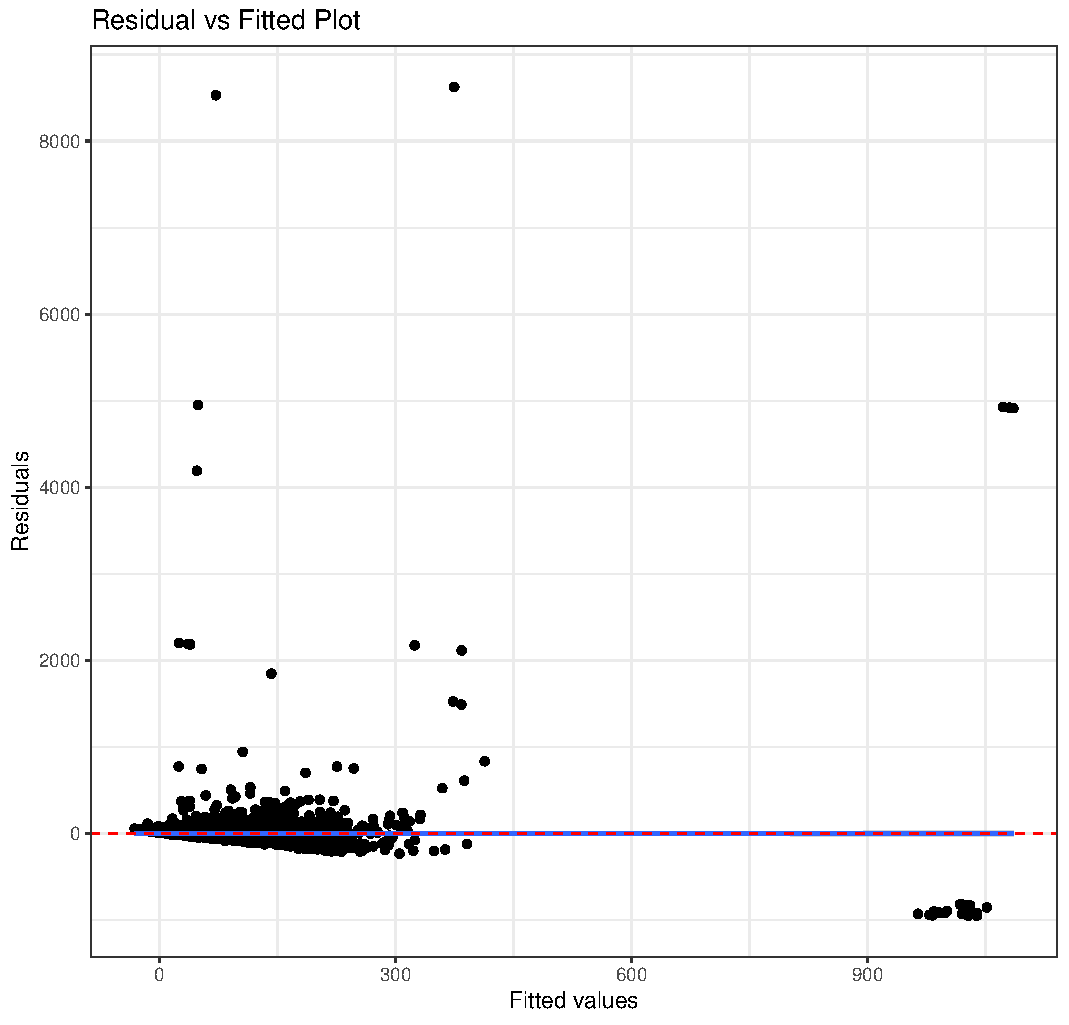
\includegraphics[height=0.5\textwidth]{fittedactual.pdf}}
\subfloat[Residuals QQ Plot]{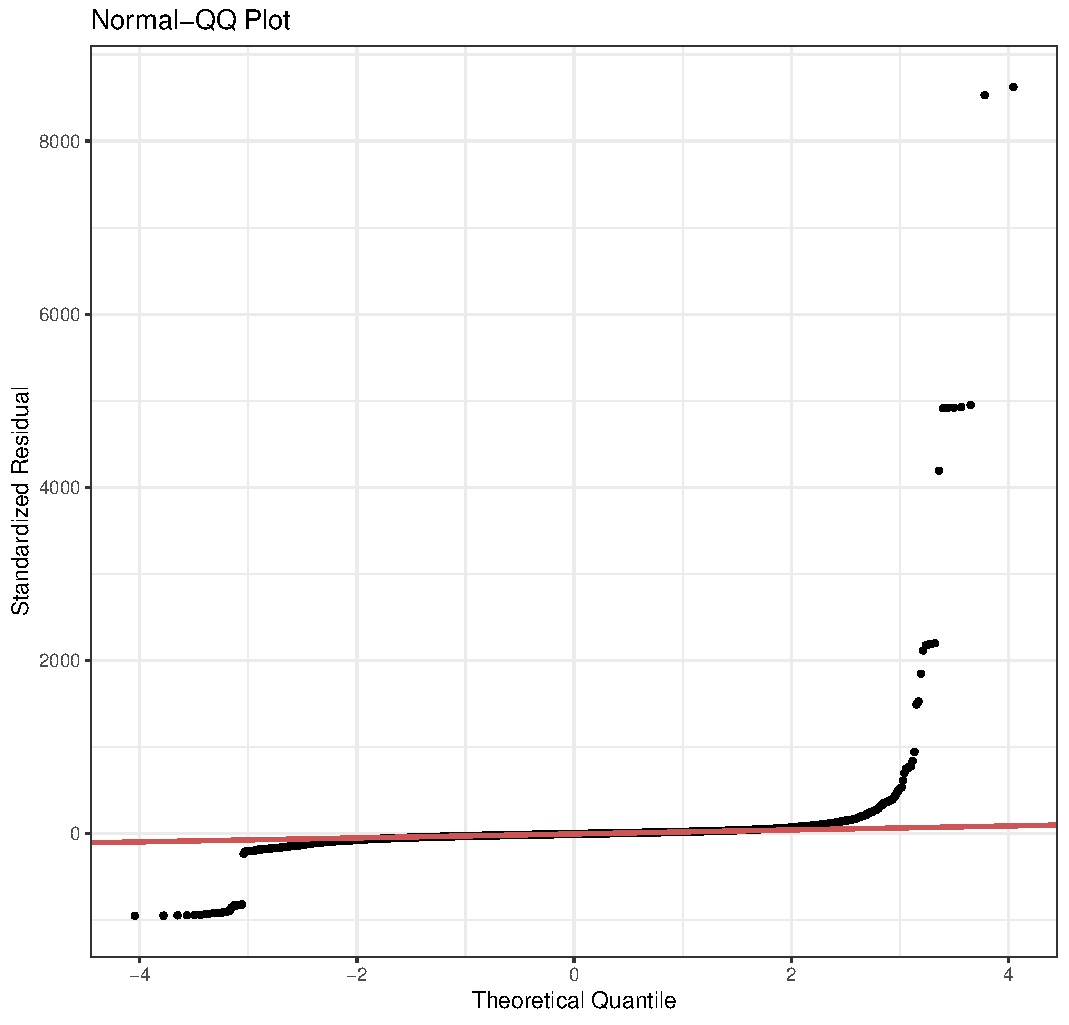
\includegraphics[height=0.5\textwidth]{qqplot.pdf}
\label{figure:cluster_plot}}
\caption{Plotting the clusters}
\label{figure:regrplots}
\centering
\end{figure}

Finally, the $R^2$ for this model, that is the proportion of the variance of \textit{price} captured by the regressors, is only 0.1298, meaning that there is much room for improvement. One can test linear regression with other variables using the ShinyApp described in \ref{Sec:shiny}.
\newpage
\section{Clustering}\label{Sec:cluster}

A further step in data analysis is clustering, that is, trying to find groups in the data where they are similar to each other but different than data in other groups  \citep{kaufman2009finding}.

In this study we tried to see if Airbnb properties in Berlin can be split into clusters sharing common features. For this purpose we will use k-means clustering, one of the most famous and used paritioning methods.

The basic ideas of this method were developed at the beginning of the second half of the $20^{th}$ century \citep{bock2007clustering}. This approach partitions the data to its closest centroid in one of the user-specified \textit{k} number of clusters. The process works according to the following steps \citep{tan2018introduction}:
\begin{enumerate}
    \item k points are randomly selected to be centroids.
    \item The rest of the data points are assigned to the respectively closest centroid, i.e. the one which minimizes the sum of the squared error (SSE)
    \begin{equation}
SSE = \sum\limits_{i=1}^{K} \sum\limits_{\textbf{x}\in C_i} dist(\textbf{c}_i, \textbf{x})^2    
	\end{equation}
where $dist(\textbf{c}_i, \textbf{x})$ is the Euclidean distance between the centroid of the $i^{th}$ cluster and a point \textbf{x}.     
    \item New centroids are selected, being the mean of all points in the respective cluster.
    \item Repeat points 2. and 3. until the centroids stop changing or the maximum number of iterations has been reached.
\end{enumerate}

Subsection \ref{subsec:numclusters} will deal with the process of choosing the appropriate number of clusters to be used in the clustering algorithm, while subsection \ref{subsec:kmeans} will handle the clustering itself.

\subsection{Choosing the number of clusters}\label{subsec:numclusters}

According to procedure explained above, the first thing to do is to choose the number of clusters \textit{k}. As illustrated in \cite{kodinariya2013review}, there are multiple approaches to selecting the appropriate value of \textit{k}. In this study the elbow method was used, since it can be calculated using the k-means algorithm and it does require too much computational power.

This method is a visual rule of thumb implemented in the function \texttt{number\_of\_clusters} and is \cite{madhulatha2012overview}. It firstly requires the user to cluster the data multiple times with increasing values of k, starting at $k = 2$.

\lstinputlisting[language=R, firstline=2, lastline=16, escapechar=|, caption={|\textbf{\href{https://github.com/silvia-ventoruzzo/SPL-WISE-2018/blob/master/Helpers/number_of_clusters.R}{number\_of\_clusters.R}}|}]{../Helpers/number_of_clusters.R}

Secondly one calculates for each run the percentage of the total variance explained. 

\lstinputlisting[language=R, firstline=17, lastline=23, firstnumber=17, escapechar=|, caption={|\textbf{\href{https://github.com/silvia-ventoruzzo/SPL-WISE-2018/blob/master/Helpers/number_of_clusters.R}{number\_of\_clusters.R}}|}]{../Helpers/number_of_clusters.R}

One then plot the total variance explained against the number of clusters and chooses the value of \textit{k} where adding another cluster does not add sufficient information \citep{madhulatha2012overview}.

\lstinputlisting[language=R, firstline=24, firstnumber = 25, escapechar=|, caption={|\textbf{\href{https://github.com/silvia-ventoruzzo/SPL-WISE-2018/blob/master/Helpers/number_of_clusters.R}{number\_of\_clusters.R}}|}]{../Helpers/number_of_clusters.R}

The resulting plot can be seen in \ref{figure:numclusterplot}. In this case there is no general best, since the value of \textit{tve} is not continually increasing.

\begin{figure}[H]
\begin{center}
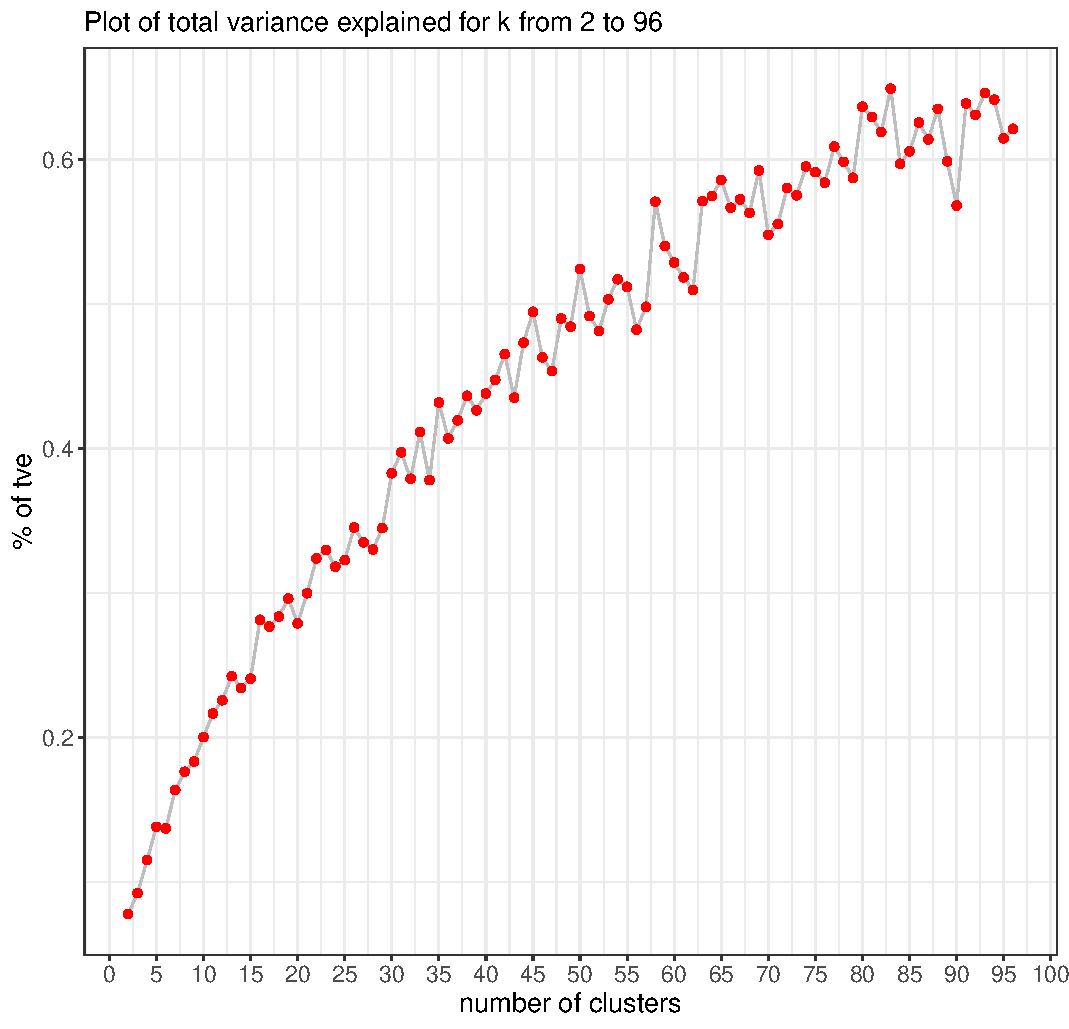
\includegraphics[width=0.8\textwidth, keepaspectratio]{numclusters.pdf} \\
\caption{Plot of the total variance explained against different values of \textit{k} \protect
\includegraphics[scale=0.05]{qletlogo.pdf} {\href{https://github.com/silvia-ventoruzzo/SPL-WISE-2018/blob/master/Helpers/number_of_clusters.R}{number\_of\_clusters.R}}}
\label{figure:numclusterplot}
\end{center}
\end{figure}

\subsection{k-means clustering}\label{subsec:kmeans}

After selecting the number of clusters to use, one can apply it inside the function \texttt{kmeans} and look at the cluster assignments of the different points.

Having multiple variables, plotting the clustered points with respect to all variables is not feasible, one need therefore to find alternatives. Since we have coordinate points, one possibility is to plot the points with respect to their longitude and latitude, like in figure .... Another one can be to plot them with respect to the first two principal components.
\section{ShinyApp}\label{Sec:shiny}

\texttt{shiny} is an \texttt{R} package that allows the user to write interactive web applications. These are especially helpful when delivering information to people with no coding experience in a very user-friedly way.

As described in the official site of \texttt{shiny}, in its most basic version an App is contained in a single script called \textit{app.R}. As the Apps become more and more complicated one can write the code in two scripts, \textit{ui.R} and \textit{server.R}, or even further split these into thematic scripts.
\\
The App structure is divided into two main elements:
\begin{itemize}
    \item \textit{ui}: The user interface object determines the appearance of the App itself. Here the possible inputs and the ouputs will be defined.
    \item \textit{server}: The server function uses the input values chosen in the App to produce the outputs indicated in the user interface. 
\end{itemize}

Finally the App will be called using the function \texttt{shinyApp(ui, server)}.

Because of its interactiveness and flexibility a ShinyApp was built for this project in order to enable the final user a chance to a first hand analysis of the data. The code for the App can be found in the Appendix at subsection \ref{subsec:codeshiny}. It is divided into four tabs: the first one is just introductory, presenting the project and the App itself; the second display Berlin maps and descriptive statistics according to section \ref{Sec:Exploratory}; the third relates to price analysis explained in section \ref{Sec:Price analysis}; the fourth and final one enables the user to perform clustering, like illustrated in section \ref{Sec:cluster}. The ShinyApp is reachable at this link: \url{https://silviav.shinyapps.io/airbnb-berlin/}.


\newpage
\section{Results and Conclusions}\label{Sec:Conc}

\begin{itemize}

    \item Give a short summary of what has been done and what has been
    found.

    \item Expose results concisely.

    \item Draw conclusions about the problem studied. What are the
    implications of your findings?

    \item Point out some limitations of study (assist reader in judging validity
    of findings).

    \item Suggest issues for future research.

\end{itemize}




% ----------------
% --- appendix ---
% ----------------
\appendix

% literature
\newpage
\addcontentsline{toc}{section}{References}
\bibliography{literature}



% --------------------------------------------
% --- last page: Declaration of Authorship ---
% --------------------------------------------

\newpage
\thispagestyle{empty}
%{\Large{\bf Declaration of Authorship}}\vspace{0.5cm}

\section*{Declaration of Authorship}

I hereby confirm that I have authored this seminar paper independently and without use of others than the indicated
sources. All passages which are literally or in general matter
taken out of publications or other sources are marked as such.
\vspace{1cm}

Berlin, \today \vspace{0.5cm}

Silvia Ventoruzzo



\end{document}
